\documentclass[lettersize,journal]{IEEEtran}
\usepackage{amsmath,amsfonts}

\usepackage{algorithm}
\usepackage{array}
\usepackage[caption=false,font=normalsize,labelfont=sf,textfont=sf]{subfig}
\usepackage{textcomp}
\usepackage{stfloats}
\usepackage{listings}
\usepackage{url}
\usepackage{verbatim}
\usepackage{graphicx}
\usepackage{cite}
\usepackage{float}
\usepackage{hyperref}
\usepackage{makecell} 
\hyphenation{op-tical net-works semi-conduc-tor IEEE-Xplore}
\usepackage{array}
\usepackage{ragged2e}
\newcolumntype{P}[1]{>{\RaggedRight\arraybackslash}p{#1}}
\usepackage{amssymb}
\usepackage{algpseudocode}
\newcommand{\xmark}{\ding{x}}
\begin{document}

\title{Enhancing Facial Emotion Recognition in Augmented Reality Using Adversarial Generative Networks for Mental Health Promotion}



\maketitle

\begin{abstract}
Facial emotion recognition (FER) in augmented reality (AR) environments faces challenges due to environmental variations such as lighting, pose, and occlusions. We propose an algorithm that integrates an adversarial generative network (AGNet) into the FER pipeline to enhance robustness. The AGNet generates identity-free facial representations, focusing on expression-related features. This approach improves emotion recognition accuracy and provides reliable AR feedback, which can significantly promote mental health by enabling real-time emotional support and interventions in varying conditions.
\end{abstract}



\section{Introduction}
\IEEEPARstart{F}{acial} Expression Recognition (FER) is a key tool for assessing emotional states, especially in the field of mental health, helping to identify conditions like depression, anxiety,  and stress that are difficult to express verbally.  FER has evolved from traditional methods,  such as Local Binary Pattern (LBP) and Histogram of Oriented Gradients (HOG), to advanced deep learning techniques,  significantly improving accuracy and efficiency.  LBP and HOG, which focus on manually extracted features,  form the foundation of FER,  with LBP detecting subtle texture changes and HOG capturing edge orientation.  With the rise of deep learning approaches  like Convolutional Neural Networks (CNNs) and Vision Transformers (ViTs),  traditional methods are increasingly being replaced,  automating feature extraction and offering higher accuracy and scalability.  This shift has enabled new opportunities  for mental health applications,  such as mood monitoring and therapeutic support.  

This paper reviews both traditional and deep learning-based FER  methods,  analyzing their strengths and limitations in mental health applications and comparing their adaptability to challenges  such as insufficient data, poor environments, and limited computing power.

\section{Traditional FER Analysis}
\label{sec:traditional_fer}

Facial Expression Recognition (FER) plays a crucial role in assessing emotional states, which is highly relevant for mental health applications. Traditional FER methods rely on handcrafted features and classical machine learning algorithms.The following is the analysis of two patterns: LBP and HOG:



\bibliographystyle{IEEEtran}

\subsection{Local Binary Patterns (LBP)}

Local Binary Patterns extract texture features by thresholding the neighborhood of each pixel~\cite{Ojala2002}. In mental health, LBP can detect subtle changes in facial expressions associated with conditions like depression or anxiety.

\begin{figure}[htbp]
    \centering
    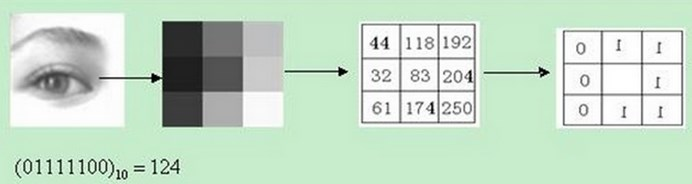
\includegraphics[width=0.7\linewidth]{Traditional FER/LBP_process.png} \\
    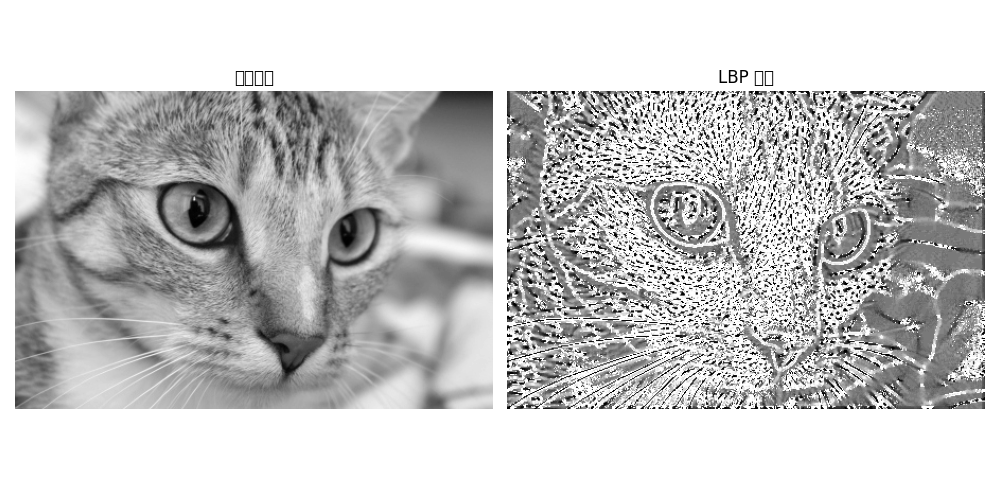
\includegraphics[width=0.7\linewidth]{Traditional FER/LBP_result.png}
    \caption{Example of LBP feature extraction process(Top).  Example of LBP feature extraction result(Bottom)\cite{van2014scikit}.}
    \label{fig:lbp_combined}
\end{figure}

\textbf{Advantages:}
\begin{itemize}
    \item \emph{Computational Efficiency:} Suitable for real-time emotion monitoring in therapeutic settings.
    \item \emph{Robustness to Illumination Changes:} Performs well under varying lighting conditions.
\end{itemize}

\textbf{Limitations:}
\begin{itemize}
    \item \emph{Lack of Global Context:} LBP operates at the pixel level by comparing each pixel to its local neighbors, which inherently restricts its ability to capture relationships across distant facial regions. As a result, it may fail to interpret complex or subtle facial expressions that require understanding the interplay between multiple facial features, such as simultaneous changes in the eyes and mouth. This limitation makes it less effective for analyzing emotional states in mental health assessments, where global context often plays a critical role.
    \item \emph{Sensitivity to Noise:} Since LBP directly processes raw pixel intensities, it is highly susceptible to image artifacts such as noise, compression errors, and blurring. Small variations in pixel values, which are common in low-quality images, can significantly alter the LBP codes.
\end{itemize}

\subsection{Histogram of Oriented Gradients (HOG)}

HOG captures edge orientations and is effective in representing facial features~\cite{Dalal2005}. It helps in identifying expressions linked to emotional states relevant in psychological evaluations.
\begin{figure}[htbp]
    \centering
    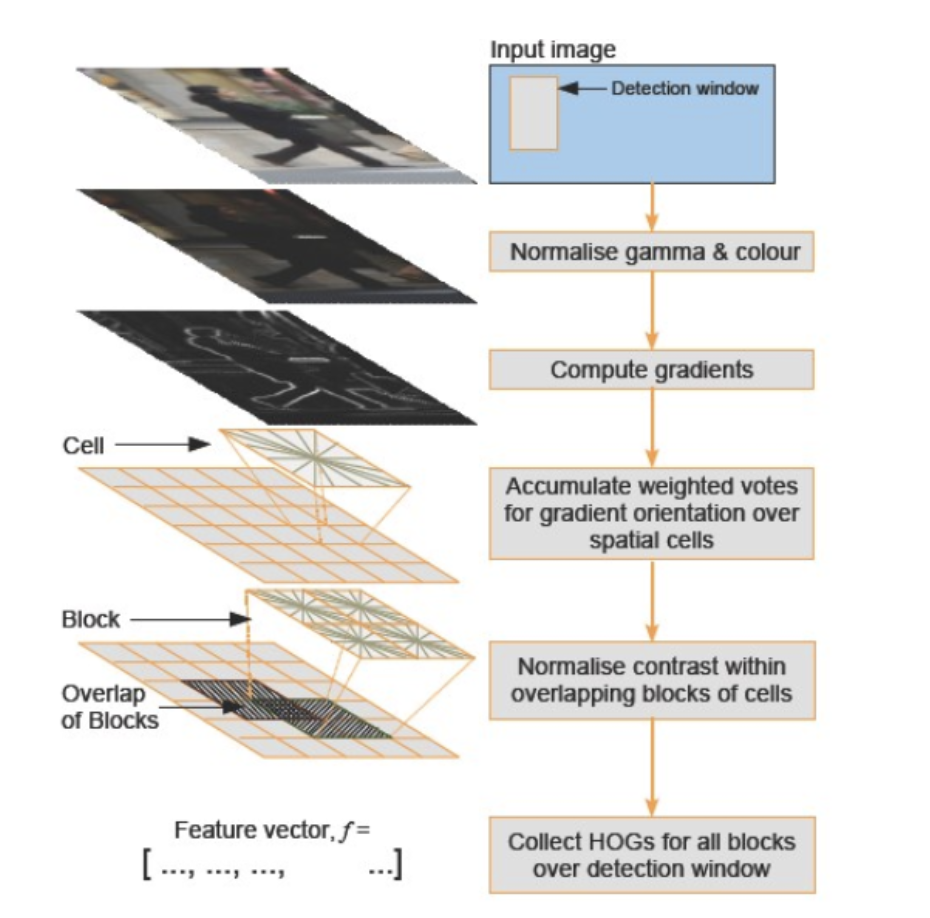
\includegraphics[width=0.7\linewidth]{Traditional FER/HOG_process.png} \\
    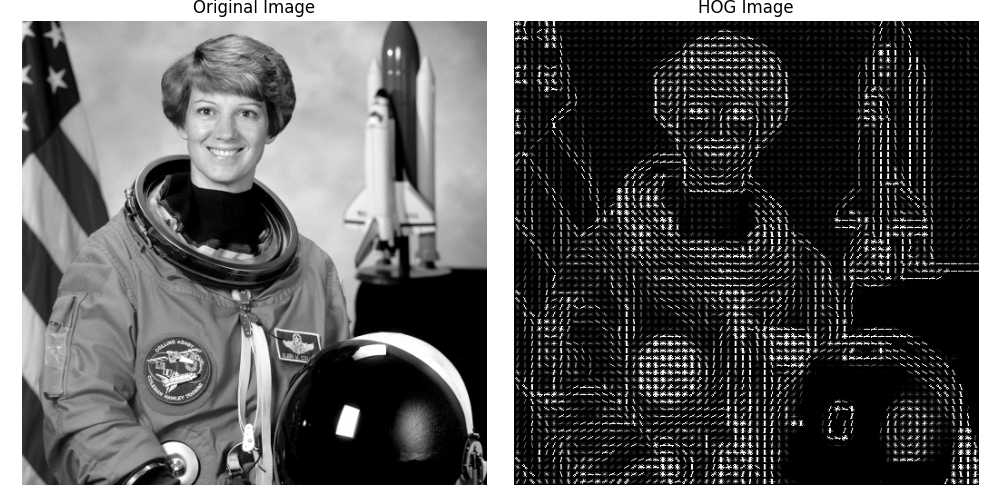
\includegraphics[width=0.7\linewidth]{Traditional FER/HOG_result.png}
    \caption{Example of HOG feature extraction process(Top).  Example of HOG feature extraction result(Bottom)\cite{van2014scikit}.}
    \label{fig:lbp_combined}
\end{figure}
\textbf{Advantages:}
\begin{itemize}
    \item \emph{Effective Feature Representation:} Captures essential facial structure information.
    \item \emph{Invariance to Geometric Transformations:} Robust against slight facial movements.
\end{itemize}

\textbf{Limitations:}
\begin{itemize}
    \item \emph{High Dimensionality:} HOG extracts features by dividing an image into small cells and calculating the histogram of gradient orientations for each cell. This process generates a large number of features, especially for high-resolution images or when fine-grained cell sizes are used. Such high-dimensional feature vectors increase the computational complexity and require dimensionality reduction techniques, such as Principal Component Analysis (PCA), to make the data manageable for classification algorithms. However, dimensionality reduction can sometimes lead to information loss, affecting the accuracy of facial expression analysis.
    \item \emph{Computational Load:} The calculation of gradient orientations, normalization across overlapping blocks, and the construction of histograms are computationally intensive. These steps involve processing a large number of pixels and performing repeated calculations for overlapping regions, significantly increasing processing time. This high computational demand makes HOG less suitable for real-time applications like mental health monitoring, where rapid feedback is essential. Additionally, when implemented on devices with limited processing power, such as wearable AR systems, this computational burden can lead to performance bottlenecks.
\end{itemize}

\section{Deep Learning-Based FER in Mental Health Support}

Facial emotion recognition (FER) has gained considerable attention in the mental health domain due to its ability to analyze non-verbal emotional cues, offering insights into a person’s psychological state. Deep learning techniques, particularly Convolutional Neural Networks (CNNs), Vision Transformers (ViTs), and hybrid models like Segmentation VGG-19, have revolutionized FER by enabling automated and highly accurate emotion classification. These advancements present significant opportunities for mental health support, including emotion monitoring, diagnosis, and therapeutic interventions~\cite{Dada2023, Vignesh2023}.

\subsection*{Advantages of Deep Learning-Based FER in Mental Health}

Deep learning models excel at identifying and classifying facial expressions by extracting complex spatial and contextual features. CNN architectures such as CNN-10 are highly effective at capturing both local and global features, achieving impressive accuracy rates, including 99.9\% on CK+ and 84.3\% on FER-2013 datasets~\cite{Dada2023}. The performance of the CNN-10 model was evaluated using accuracy, precision, recall, and F1-score, computed as follows:

\begin{equation}
\text{F1-score} = 2 \cdot \frac{\text{Precision} \cdot \text{Recall}}{\text{Precision} + \text{Recall}},
\label{eq:f1_score}
\end{equation}
where precision and recall are given by:
\begin{equation}
\text{Precision} = \frac{\text{True Positives}}
{\text{True Positives} + \text{False Positives}},
\label{eq:precision}
\end{equation}

\begin{equation}
\text{Recall} = \frac{\text{True Positives}}
{\text{True Positives} + \text{False Negatives}}.
\label{eq:recall}
\end{equation}

A summary of CNN-10's performance on different datasets is presented in Table~\ref{tab:cnn10_performance}, demonstrating its robustness and high accuracy in controlled settings.

\begin{table}[h!]
\centering
\caption{Performance of CNN-10 on various datasets~\cite{Dada2023}.}
\label{tab:cnn10_performance}
\begin{tabular}{|c|c|c|c|c|}
\hline
\textbf{Dataset} & \textbf{Accuracy (\%)} & \textbf{Precision} & \textbf{Recall} & \textbf{F1-score} \\ \hline
CK+              & 99.9                  & 0.99              & 0.99            & 0.99              \\ \hline
FER-2013         & 84.3                  & 0.85              & 0.84            & 0.84              \\ \hline
JAFFE            & 95.4                  & 0.96              & 0.95            & 0.95              \\ \hline
\end{tabular}
\end{table}

The inclusion of ViTs further enhances performance by leveraging self-attention mechanisms to understand the relationships between various facial regions, providing a holistic understanding of expressions~\cite{Dada2023}.\\
Although deep learning excels in facial recognition, challenges like inefficient long-range dependency capture and gradient vanishing in deep networks remain. Attention mechanisms address these issues by guiding models to focus on key regions (e.g., eyes, mouth) rather than the entire face, enhancing efficiency and performance.

Attention-based convolutional neural networks (ACNNs) effectively handle facial occlusion by focusing on symmetric regions to capture essential features even when parts are obscured. Y. Li et al. (2019) demonstrated that ACNNs improve facial expression recognition under occlusion, boosting robustness and accuracy \cite{Li2019}.

The feature relationship can be expressed as:
\[
F = X \otimes (1 + S)
\]
\( F \) is the final output, \( X \) the input feature map, and \( S \) the attention-enhanced features. This highlights how attention refines feature representation by emphasizing critical areas.

In conclusion, attention-guided CNNs improve facial recognition, especially in occluded and complex real-world conditions.

\subsection*{Limitations of Current FER Technology}

\begin{enumerate}
    \item \textbf{Sensitivity to Environmental Variations}: Deep learning-based FER models struggle with real-world changes like lighting, occlusions, and diverse poses, leading to reduced accuracy in uncontrolled settings~\cite{Dada2023, Vignesh2023}. Large, diverse datasets are required, but real-world variations still pose challenges.
    
    \item \textbf{Dataset Imbalance}: Imbalanced datasets, such as FER-2013 with underrepresented emotions like "disgust," limit the generalizability of models~\cite{Vignesh2023}. This bias affects their ability to detect subtle or rare emotional states, critical in mental health applications.
    
    \item \textbf{Overfitting}: Limited or biased data often causes overfitting, making models excel on training data but fail to generalize to unseen scenarios, reducing reliability in diverse settings~\cite{Dada2023}.
    
    \item \textbf{High Computational Demands}: Models like Segmentation VGG-19 require significant resources, making them impractical for real-time or low-resource environments~\cite{Vignesh2023}. Optimization techniques help but cannot fully resolve this issue.
    
    \item \textbf{Lack of Interpretability}: Deep learning models function as "black boxes," limiting trust in clinical applications~\cite{Dada2023}. Transparent models are essential for ensuring adoption in sensitive environments like mental health care.
\end{enumerate}



\subsection*{Critical Analysis and Future Directions}

Deep learning-based FER has significant potential in mental health for early diagnosis, personalized therapy, and ongoing emotional monitoring. To realize its full impact, researchers must focus on creating diverse datasets, optimizing model efficiency for real-time applications, and enhancing interpretability to ensure clinical reliability and usability~\cite{Dada2023, Vignesh2023}.\\


To address the challenge of creating diverse data sets, data enhancement techniques offer a powerful solution. By enhancing the available data sets, these techniques allow for the generation of larger and more diverse sets of training images, which is critical for deep learning models that require large amounts of data to avoid overfitting. ~\cite{Akhand2021} highlights the effectiveness of geometric transformations such as random rotations, translations, and flips, as well as more advanced methods such as generative adversarial networks (GANs). These enhancement strategies have been shown to significantly improve model accuracy, particularly with the combination of generative adversarial networks and geometry techniques increasing recognition accuracy from 0.53 to 0.75, and also from 0.15 to 0.40 in complex cases.




\section{Vertical contrast of all FER}

\begin{table}[H]
\caption{Extended Performance Comparison of FER Models (Vertical Layout)}
\label{tab:model_comparison_extended}
\centering
\footnotesize
\begin{tabular}{|p{1.6cm}|p{0.7cm}|p{0.7cm}|p{0.7cm}|p{0.7cm}|p{0.7cm}|p{0.7cm}|}
\hline
\textbf{Criteria}              & \textbf{LBP} & \textbf{HOG} & \textbf{CNNs} & \textbf{VGG-19} & \textbf{U-Net} & \textbf{ViTs} \\
\hline
Invention Year        & 1994         & 2005         & 1989 / 2012  & 2014            & 2015           & 2020          \\
\hline
Application Year      & 2002         & 2005--2010   & 2012--2015   & 2015            & 2015--2017     & 2020-- \\
\hline
Computational Complexity & 1           & 2            & 6            & 5               & 4              & 3             \\
\hline
Robustness            & 6           & 5            & 4            & 3               & 2              & 1             \\
\hline
Interpretability      & Good        & Good         & Bad          & Bad             & Medium         & Medium        \\
\hline
Training Time         & Fast        & Medium       & Slow         & Very Slow       & Medium         & Slow          \\
\hline
Inference Speed       & Fast        & Fast         & Medium       & Medium          & Slow           & Medium        \\
\hline
Energy Efficiency     & High        & High         & Medium       & Low             & Medium         & Medium        \\
\hline
Data Requirements     & 1           & 2            & 6            & 5               & 3              & 4             \\
\hline
Real-time Performance & 1           & 2            & 6            & 5               & 4              & 3             \\
\hline
Scalability           & 6           & 5            & 1            & 2               & 3              & 4             \\
\hline
Cross-Cultural Adaptability & Medium     & Medium       & High         & High            & High           & High          \\
\hline
Integration Complexity & Low         & Medium       & High         & Very High       & Medium         & Medium        \\
\hline
\end{tabular}

\begin{flushleft}
\textbf{Ranking Rules}: 
\begin{itemize}
    \item A lower number indicates better performance for the specific criterion.
    \item \textbf{1}: Best performance.
    \item \textbf{6}: Worst performance.
    \item Rankings are relative, determined based on the comparative strengths and weaknesses of the models.
\end{itemize}
\textbf{Descriptions for Non-Ranking Criteria}:
\begin{itemize}
    \item \textbf{Interpretability}: \textbf{Good} = easy to explain; \textbf{Medium} = partially explainable; \textbf{Bad} = difficult to interpret.
    \item \textbf{Training Time}: \textbf{Fast} <1 hour, \textbf{Medium} 1--3 hours, \textbf{Slow} >3 hours, \textbf{Very Slow} >10 hours.
    \item \textbf{Energy Efficiency}: \textbf{High} = suitable for low-power devices, \textbf{Medium} = moderate energy requirements, \textbf{Low} = energy-intensive.
    \item \textbf{Cross-Cultural Adaptability}: How well the model generalizes across different cultural datasets.
    \item \textbf{Integration Complexity}: \textbf{Low} = easily integrated, \textbf{Medium} = moderate integration effort, \textbf{High} = requires significant effort, \textbf{Very High} = very challenging to integrate.
\end{itemize}
\end{flushleft}

\end{table}

\section{Segmentation Technology Analysis}
\label{sec:segmentation_analysis}

Accurate facial segmentation is essential for isolating regions of interest, improving the reliability of FER in mental health assessments.

\subsection{Active Contour Models (Snakes)}

Active Contour Models detect object boundaries by minimizing an energy function~\cite{Kass1988}. In mental health applications, they help in accurately delineating facial features to analyze emotional expressions.
\begin{figure}[H]
    \centering
    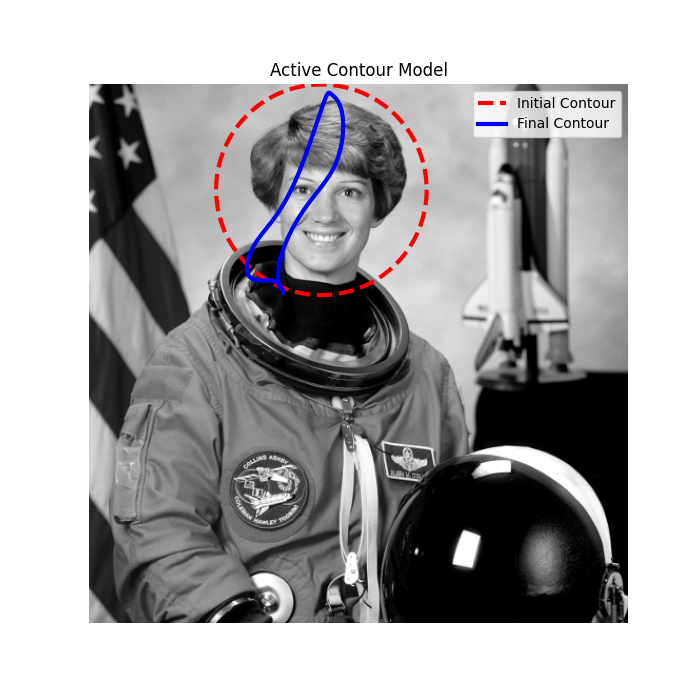
\includegraphics[width=0.7\linewidth]{Traditional FER/Active Contour Model.png} \\
    
    \caption{Example result of Active Contour Models\cite{van2014scikit}}
    \label{fig:lbp_combined}
\end{figure}
\textbf{Advantages:}
\begin{itemize}
    \item \emph{Precision in Boundary Detection:} Facilitates detailed analysis of facial movements.
    \item \emph{Flexibility:} Adapts to various facial shapes and expressions.
\end{itemize}

\textbf{Limitations:}
\begin{itemize}
    \item \emph{Initialization Sensitivity:} Requires good initial contours to converge properly.
    \item \emph{Computational Intensity:} May not be suitable for real-time processing needed in mental health interventions.
\end{itemize}

\subsection{Deep Learning-based Segmentation (U-Net Architecture)
}
Deep learning-based segmentation methods, particularly U-Net, have gained significant attention in recent years for their ability to accurately segment complex objects in images, including human faces. U-Net is a convolutional neural network (CNN) architecture designed for image segmentation, featuring a symmetric encoder-decoder structure. It has been successfully applied in facial expression recognition (FER) and psychological analysis.~\cite{Ibtehaz2020}

\textbf{Advantages:}
\begin{itemize}
    \item \emph{Precision in Boundary Detection:} Facilitates detailed analysis of facial movements.
    \item \emph{Flexibility:} Adapts to various facial shapes and expressions.
\end{itemize}

\textbf{Limitations:}
\begin{itemize}
    \item \emph{Initialization Sensitivity:} Requires good initial contours to converge properly.
    \item \emph{Computational Intensity:} May not be suitable for real-time processing needed in mental health interventions.
\end{itemize}

\subsection{Watershed Segmentation}

Watershed algorithms treat the image as a topographic surface for region segmentation~\cite{Meyer1994}. They can segment facial regions to enhance FER accuracy in psychological diagnostics.
\begin{figure}[H]
    \centering
    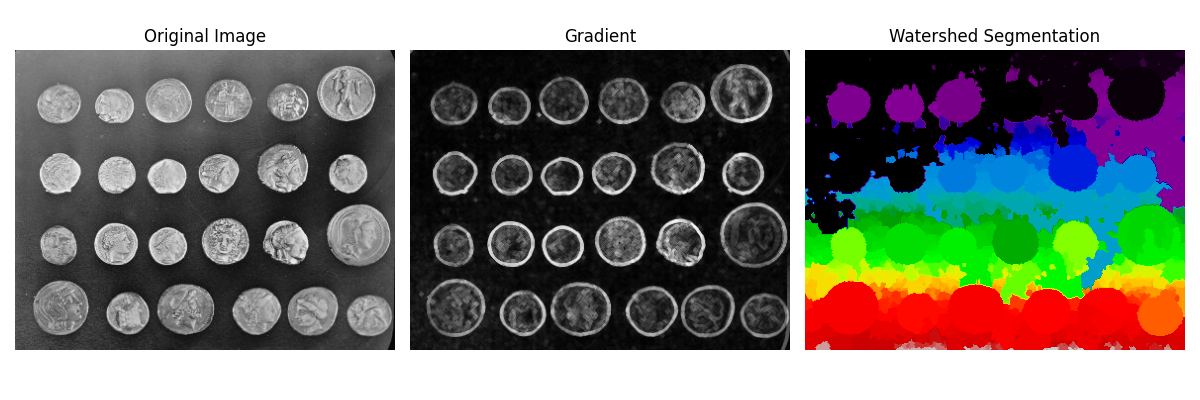
\includegraphics[width=0.7\linewidth]{Traditional FER/Watershed Segmentation.png} \\
    
    \caption{Example result of Watershed Segmentation\cite{van2014scikit}}
    \label{fig:lbp_combined}
\end{figure}
\textbf{Advantages:}
\begin{itemize}
    \item \emph{Detailed Segmentation:} Capable of separating adjacent facial features effectively.
    \item \emph{No Requirement for Edge Detection:} Operates on gradient information.
\end{itemize}

\textbf{Limitations:}
\begin{itemize}
    \item \emph{Over-segmentation Risk:} May produce excessive regions, complicating the analysis.
    \item \emph{Noise Sensitivity:} Requires preprocessing steps to reduce image noise.
\end{itemize}


\section{Limitations of FER Algorithms}
\label{sec:limitations}

Facial Expression Recognition (FER) algorithms have advanced significantly but still face several limitations that affect their performance, especially in mental health applications. This section summarizes these shortcomings by grouping similar issues, analyzing their severity, and proposing potential solutions.

\subsection{Sensitivity to Environmental Conditions}

\textbf{Common Problem:} FER algorithms are highly sensitive to variations in lighting, facial poses, and occlusions (e.g., glasses, masks). Changes in these conditions can significantly degrade the performance of both traditional and deep learning-based models, as they rely heavily on visual cues that may be distorted or obscured.

\textbf{Severity Analysis:} This issue is severe because it directly impacts the reliability and accuracy of emotion recognition in real-world settings. In mental health support, where accurate detection of subtle emotional cues is crucial, any inconsistency due to environmental factors can lead to misinterpretation and ineffective interventions.

\textbf{Proposed Solutions:}
	•	\emph{Data Augmentation with GANs:} Utilize Generative Adversarial Networks (GANs) to generate synthetic images under various environmental conditions. This can help in training models to be more robust to changes in lighting, pose, and occlusions by exposing them to a wider range of scenarios~\cite{Akhand2021}.
	•	\emph{Attention Mechanisms:} Incorporate attention mechanisms in neural networks to focus on essential facial regions less affected by environmental variations, enhancing the model’s ability to extract relevant features~\cite{Li2019}.
	•	\emph{Preprocessing Techniques:} Apply image normalization and enhancement methods to reduce the impact of lighting variations and improve feature consistency across different conditions.

\subsection{Data Dependency and Dataset Limitations}

\textbf{Common Problem:} Deep learning-based FER models require large, diverse, and well-annotated datasets to perform effectively. However, available datasets often suffer from class imbalances, lack of diversity, and insufficient sample sizes, especially for underrepresented emotions.

\textbf{Severity Analysis:} This limitation is critical as it leads to biased models that may not generalize well to new data. In mental health applications, where recognizing a wide spectrum of emotions is essential, such biases can result in inaccurate assessments.

\textbf{Proposed Solutions:}
	•	\emph{Data Augmentation:} Implement techniques like rotation, scaling, flipping, and adding noise to existing images to artificially increase dataset size and diversity.
	•	\emph{Synthetic Data Generation with GANs:} Use GANs to create synthetic images of underrepresented emotions, helping to balance the dataset and improve model generalization.
	•	\emph{Transfer Learning:} Leverage pre-trained models on large datasets and fine-tune them on specific FER tasks to mitigate the impact of limited data.

\subsection{Computational Complexity}

\textbf{Common Problem:} Advanced FER algorithms, particularly deep learning models like CNNs, Vision Transformers (ViTs), and segmentation networks like VGG-19, demand high computational resources for both training and inference.

\textbf{Severity Analysis:} This issue is significant because it hinders the deployment of FER systems in real-time applications and on devices with limited processing capabilities, such as mobile phones or augmented reality (AR) glasses used in mental health interventions.

\textbf{Proposed Solutions:}
	•	\emph{Model Optimization:} Employ model compression techniques such as pruning, quantization, and knowledge distillation to reduce the computational load without substantially sacrificing accuracy.
	•	\emph{Lightweight Architectures:} Design and utilize efficient neural network architectures tailored for low-resource environments, like MobileNet or SqueezeNet.
	•	\emph{Edge Computing:} Implement edge computing strategies to process data locally, reducing latency and reliance on centralized servers.

\subsection{Overfitting}

\textbf{Common Problem:} FER models are prone to overfitting, where they perform exceptionally well on training data but poorly on unseen data. This occurs due to complex models being trained on limited or non-representative datasets.

\textbf{Severity Analysis:} Overfitting severely limits the practical applicability of FER models, as they fail to generalize to real-world scenarios. In mental health support, this can lead to incorrect emotion recognition, affecting the quality of care provided.

\textbf{Proposed Solutions:}
	•	\emph{Regularization Techniques:} Apply methods like dropout, weight decay, and data augmentation during training to prevent overfitting.
	•	\emph{Cross-Validation:} Use k-fold cross-validation to ensure the model’s robustness across different subsets of data.
	•	\emph{Simplifying Models:} Reduce model complexity by limiting the number of layers or parameters to match the amount of available data.

\subsection{Limitations of Traditional Methods}

\textbf{Common Problem:} Traditional FER methods like Local Binary Patterns (LBP) and Histogram of Oriented Gradients (HOG) focus on handcrafted features and often fail to capture the global context of facial expressions.


\textbf{Severity Analysis:} This limitation is moderate but still important. The inability to consider the overall facial structure reduces the effectiveness of these methods in recognizing complex or subtle emotions, which are crucial in mental health assessments.

\textbf{Proposed Solutions:}
	•	\emph{Hybrid Approaches:} Combine traditional feature extraction methods with deep learning techniques to leverage the strengths of both.
	•	\emph{Feature Fusion:} Integrate multiple feature descriptors to capture both local and global facial information.
	•	\emph{Transition to Deep Learning:} Gradually adopt deep learning models that inherently learn hierarchical features representing both local and global contexts.

\section{Proposed Algorithm Incorporating Adversarial Generative Networks for FER in AR}
\label{sec:proposed_algorithm_gan}

To address the sensitivity of Facial Emotion Recognition (FER) systems to environmental conditions, we propose an algorithm that integrates an adversarial generative network into the FER pipeline within an Augmented Reality (AR) environment. This approach enhances the robustness of emotion recognition by generating identity-free facial representations, mitigating the impact of variations in lighting, pose, and occlusions common in real-world settings.

\subsection{Algorithm Overview}

The proposed algorithm comprises the following key components:

\begin{enumerate}
\item \textbf{Image Acquisition}: Capture real-time facial images using the AR device’s camera.
\item \textbf{Preprocessing}: Normalize and align the captured images to standardize input data.
\item \textbf{Adversarial Generative Network (AGNet)}: Employ a neural style transfer generative adversarial network to generate identity-free facial images, focusing on expression-related features.
\item \textbf{Emotion Recognition}: Classify the processed images into specific emotions using a convolutional neural network (CNN).
\item \textbf{AR Feedback Integration}: Display visual cues or interventions based on the detected emotions within the AR interface.
\end{enumerate}

\subsection{Adversarial Generative Network (AGNet)}

The core component is the AGNet, designed to disentangle identity-related features from expression-related features. By generating identity-free images, the model reduces sensitivity to environmental variations.

\subsubsection{Architecture of AGNet}

The AGNet consists of a generator $G$ and a discriminator $D$, forming an adversarial framework.

\begin{figure}[htbp]
\centering
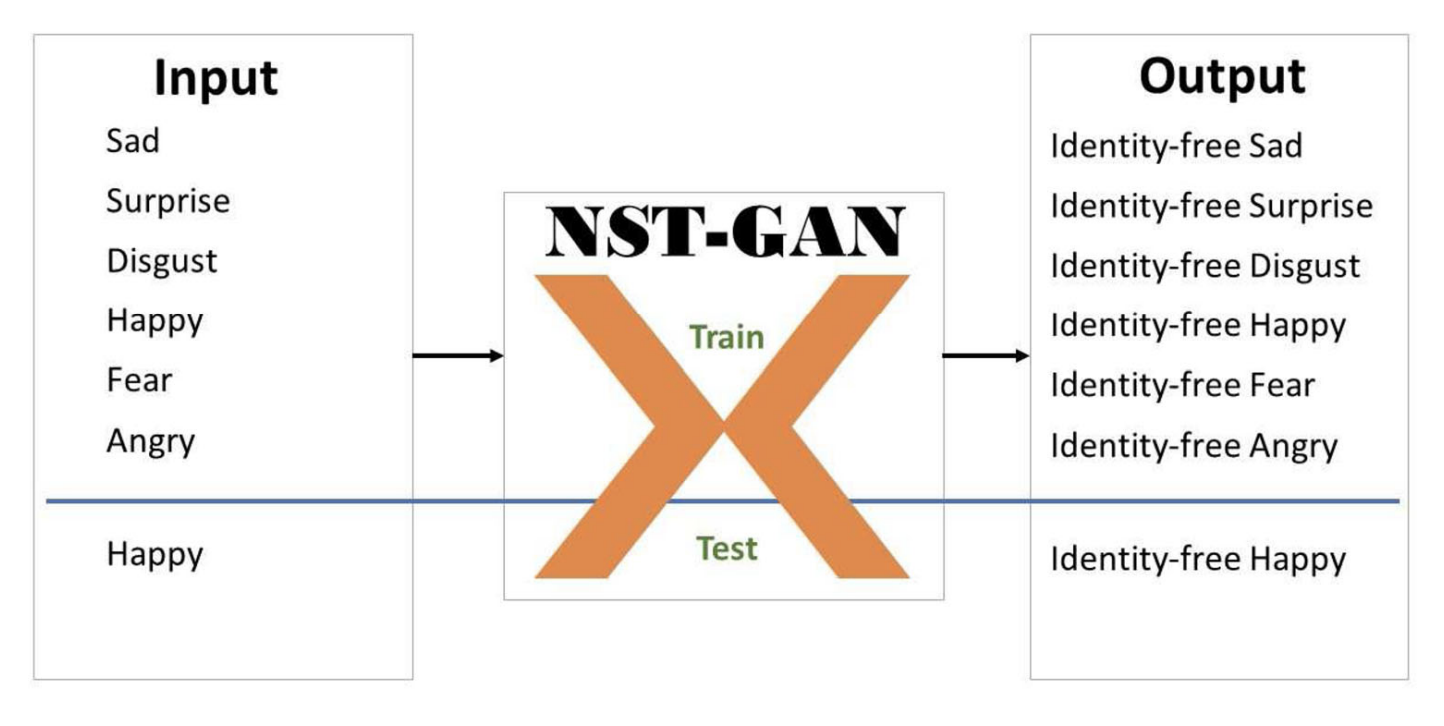
\includegraphics[width=0.8\linewidth]{AGNet_Architecture.png}
\caption{Architecture of the Adversarial Generative Network (AGNet) with generator $G$ and discriminator $D$.}
\label{fig:agnet_architecture}
\end{figure}

\textbf{Description of Figure~\ref{fig:agnet_architecture}}: The figure illustrates the AGNet where the generator $G$ takes an input image $I$ and produces an identity-free image $I’$. The discriminator $D$ attempts to distinguish between real and generated identity-free images.

\paragraph{Generator $G$}

The generator is an encoder-decoder network with skip connections (similar to U-Net). It transforms the input image $I$ into an identity-free image $I’ = G(I)$, preserving expression-related features while removing identity information.

\paragraph{Discriminator $D$}

The discriminator is a CNN that differentiates between real identity-free images and those generated by $G$. It outputs a probability $D(I’)$ indicating whether $I’$ is a real identity-free image.

\subsubsection{Loss Functions}

The AGNet is trained using a combination of adversarial loss and content loss to ensure realism and preservation of expression features.

\paragraph{Adversarial Loss}

The adversarial loss encourages $G$ to produce images indistinguishable from real identity-free images:

\begin{equation}
\mathcal{L}{\text{adv}} = \mathbb{E}{I \sim p_{\text{data}}} [\log D(I)] + \mathbb{E}{I \sim p{\text{data}}} [\log(1 - D(G(I)))]
\end{equation}

\paragraph{Content Loss}

The content loss ensures the generated image retains the expression features of the input:

\begin{equation}
\mathcal{L}{\text{content}} = \mathbb{E}{I \sim p_{\text{data}}} \left[ | \phi(I) - \phi(G(I)) |_2^2 \right]
\end{equation}

where $\phi(\cdot)$ represents feature mappings from a pre-trained network (e.g., VGG-19).

\paragraph{Total Generator Loss}

The total loss for the generator is:

\begin{equation}
\mathcal{L}{G} = \mathcal{L}{\text{adv}} + \lambda \mathcal{L}_{\text{content}}
\end{equation}

where $\lambda$ balances the adversarial and content losses.

\subsubsection{Training Procedure}

Training involves iteratively updating $G$ and $D$:

\begin{enumerate}
\item \textbf{Update Discriminator $D$}:
\begin{equation}
\max_{D} ; \mathcal{L}{\text{adv}}
\end{equation}
\item \textbf{Update Generator $G$}:
\begin{equation}
\min{G} ; \mathcal{L}_{G}
\end{equation}
\end{enumerate}

\subsection{Emotion Recognition Module}

The identity-free images $I’$ are fed into a CNN for emotion classification.

\subsubsection{CNN Architecture}

A lightweight CNN ensures real-time performance. It includes convolutional layers with batch normalization and ReLU activations, followed by pooling layers and fully connected layers for classification.

\subsubsection{Classification Process}

The emotion label $E$ is predicted as:

\begin{equation}
E = \arg\max_{k} \left( \text{Softmax}(\text{CNN}(I’)) \right)
\end{equation}

where $k$ indexes the set of emotion categories.

\subsection{Integration into AR Environment}

Based on the detected emotion, the system provides immediate feedback through the AR interface.

\subsubsection{Visual Feedback Mechanism}

Visual cues (e.g., emojis, color overlays) are displayed to the user, corresponding to their emotional state.

\subsubsection{System Workflow}

\begin{figure}[htbp]
\centering
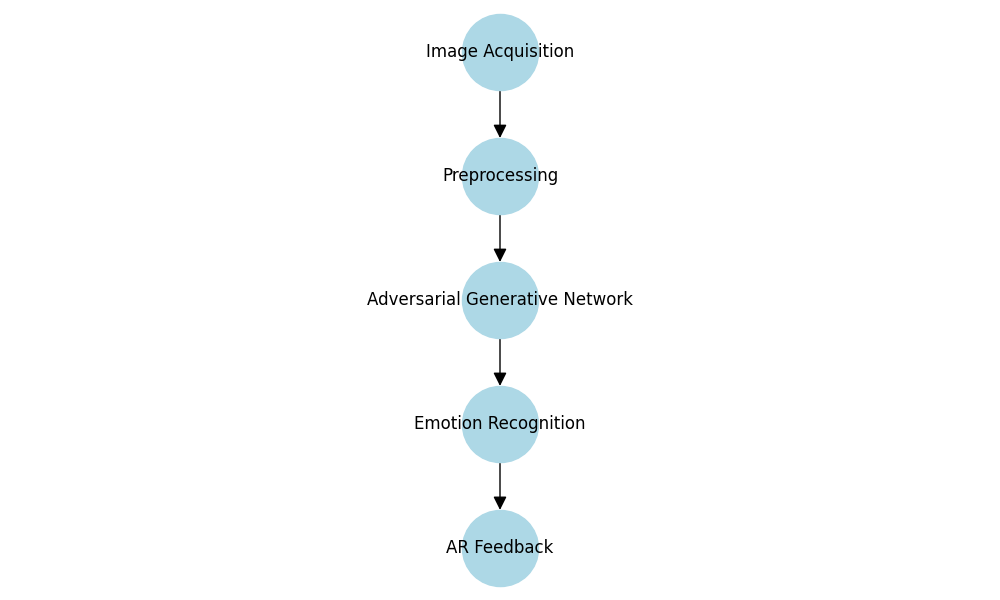
\includegraphics[width=0.9\linewidth]{System_Workflow.png}
\caption{Workflow of the proposed algorithm integrating AGNet in an AR environment.}
\label{fig:system_workflow}
\end{figure}

\textbf{Description of Figure~\ref{fig:system_workflow}}: The figure shows the sequential process starting from image acquisition, preprocessing, AGNet processing, emotion recognition, to AR feedback.

\subsection{Algorithm Advantages}

\begin{itemize}
\item \textbf{Robustness to Environmental Variations}: The AGNet reduces sensitivity to lighting, pose, and occlusions.
\item \textbf{Real-Time Performance}: Optimized architectures ensure efficiency suitable for AR applications.
\item \textbf{Enhanced Emotion Recognition}: By focusing on expression features, the algorithm improves accuracy.
\end{itemize}

\subsection{Implementation Details}

\subsubsection{Tools and Technologies}

\begin{itemize}
\item \textbf{Deep Learning Frameworks}: TensorFlow or PyTorch for implementing neural networks.
\item \textbf{Computer Vision Library}: OpenCV for image processing tasks.
\item \textbf{AR Development Kits}: ARCore (Android) or ARKit (iOS) for AR integration.
\item \textbf{Hardware Considerations}: Utilize GPUs or mobile AI accelerators for performance optimization.
\end{itemize}

\subsubsection{Data Preparation}

\begin{itemize}
\item \textbf{Dataset}: A diverse set of facial images with various expressions and environmental conditions.
\item \textbf{Data Augmentation}: Techniques such as rotation, scaling, and flipping to enhance dataset diversity.
\end{itemize}

\subsection{Considerations and Future Work}

\begin{itemize}
\item \textbf{Computational Resources}: While optimized, AGNet may still be demanding; future work could explore model compression.
\item \textbf{Privacy Concerns}: Implement on-device processing and data encryption to address privacy issues.
\item \textbf{Model Generalization}: Further research needed to improve cross-cultural and demographic adaptability.
\item \textbf{Extended Modalities}: Incorporate additional data (e.g., speech, physiological signals) to enrich emotion recognition.
\end{itemize}

\subsection{Algorithm Pseudocode}

\begin{algorithm}[htbp]
\caption{FER with Adversarial Generative Network in AR}
\label{alg:fer_agnet}
\begin{algorithmic}[1]
\While{Application is running}
\State Capture image $I$ from AR device camera.
\State Preprocess $I$ (normalization, alignment).
\State Generate identity-free image $I’ = G(I)$.
\State Classify emotion $E = \text{CNN}(I’)$.
\State Display AR feedback based on $E$.
\EndWhile
\end{algorithmic}
\end{algorithm}

\subsection{Conclusion}

Integrating an adversarial generative network into facial emotion recognition systems within augmented reality environments significantly enhances robustness against challenges like lighting variations, pose changes, and occlusions. By focusing on extracting expression-related features and generating identity-free facial representations, the improved algorithm increases the accuracy and reliability of emotion recognition.

This advancement holds substantial potential for promoting mental health. Real-time and accurate emotion recognition allows the AR system to provide immediate and appropriate feedback or interventions—such as displaying calming visuals or suggesting relaxation techniques when signs of stress or anxiety are detected. By consistently supporting users in managing their emotions across various conditions, the system contributes positively to their overall mental well-being.


\begin{thebibliography}{1}



\bibitem{Ojala2002}
T.~Ojala, M.~Pietik\"ainen, and T.~M\"aenp\"a\"a, ``Multiresolution gray-scale and rotation invariant texture classification with local binary patterns,'' \emph{IEEE Transactions on Pattern Analysis and Machine Intelligence}, vol.~24, no.~7, pp. 971--987, 2002.

\bibitem{Dalal2005}
N.~Dalal and B.~Triggs, ``Histograms of oriented gradients for human detection,'' in \emph{Proceedings of the IEEE Conference on Computer Vision and Pattern Recognition}, 2005, pp. 886--893.

\bibitem{van2014scikit}
S.~van~der~Walt, J.~L.~Schoenberger, J.~Nunez-Iglesias, F.~Boulogne, J.~D.~Warner, N.~Yager, E.~Gouillart, and T.~Yu, ``scikit-image: image processing in Python,'' \emph{PeerJ}, vol.~2, pp.~e453, 2014, doi:10.7717/peerj.453.




\bibitem{Dada2023}
E.~G.~Dada, D.~O.~Oyewola, S.~B.~Joseph, O.~Emebo, and O.~O.~Oluwagbemi, 
``Facial emotion recognition and classification using the convolutional neural network‐10 (CNN‐10),'' 
\emph{Applied Computational Intelligence and Soft Computing}, vol.~2023, Article ID 2457898, pp. 1--19, 2023.

\bibitem{Vignesh2023}
S.~Vignesh, M.~Savithadevi, M.~Sridevi, and R.~Sridhar, 
``A novel facial emotion recognition model using segmentation VGG-19 architecture,'' 
\emph{International Journal of Information Technology}, vol.~15, no.~4, pp. 1777--1787, 2023.

\bibitem{Meyer1994}
F.~Meyer, ``Topographic distance and watershed lines,'' \emph{Signal Processing}, vol.~38, no.~1, pp. 113--125, 1994.
\bibitem{Ibtehaz2020}
N.~Ibtehaz and M.~S.~Rahman, ``MultiResUNet: Rethinking the U-Net architecture for multimodal biomedical image segmentation,'' \emph{Neural Networks}, vol.~121, pp. 74--87, 2020, doi: \href{https://doi.org/10.1016/j.neunet.2019.08.025}{10.1016/j.neunet.2019.08.025}.

\bibitem{Akhand2021}
M.~A.~H.~Akhand, M.~A.~I.~Sikder, M.~S.~Rahman, and M.~A.~Haque,
``Facial Emotion Recognition Using Transfer Learning in the Deep CNN,’’
\emph{Electronics}, vol.~10, no.~9, pp. 1036, 2021.

\bibitem{Li2019}
Y.~Li, J.~Zeng, S.~Shan, and X.~Chen,
``Occlusion Aware Facial Expression Recognition Using CNN With Attention Mechanism,’’
\emph{IEEE Transactions on Image Processing}, vol.~28, no.~5, pp.~2439–2450, May 2019.

\bibitem{Goodfellow2014}
I.~Goodfellow \emph{et al.}, ``Generative adversarial nets,’’ in \emph{Advances in Neural Information Processing Systems}, 2014, pp. 2672–2680.

\bibitem{Ronneberger2015}
O.~Ronneberger, P.~Fischer, and T.~Brox, ``U-Net: Convolutional networks for biomedical image segmentation,’’ in \emph{International Conference on Medical Image Computing and Computer-Assisted Intervention}, 2015, pp. 234–241.

\bibitem{Isola2017}
P.~Isola, J.-Y.~Zhu, T.~Zhou, and A.~A.~Efros, ``Image-to-image translation with conditional adversarial networks,’’ in \emph{Proceedings of the IEEE Conference on Computer Vision and Pattern Recognition}, 2017, pp. 1125–1134.


\end{thebibliography}



\vfill


\end{document}


